% !TEX root = ../main.tex
\chapter{Bayesian Learning}
\label{ch:bayesian}

\begin{intuition}[title=\textbf{Parameters as Random Variables}]
In the frequentist paradigm, model parameters $\bm{\theta}$ are fixed but unknown quantities. The Bayesian paradigm treats $\bm{\theta}$ as a random variable endowed with a \emph{prior} distribution $p(\bm{\theta})$. Observing data $\mathcal{D}$ updates this belief to a \emph{posterior} $p(\bm{\theta}\mid\mathcal{D})$ via Bayes' theorem. The payoff: principled uncertainty quantification, automatic complexity control, and coherent model comparison.
\end{intuition}

%% ----------------------------------------------------------------
\section{Bayesian Inference}

\begin{theorem}[Bayes' Theorem]
\[
  p(\bm{\theta}\mid\mathcal{D})
  = \frac{p(\mathcal{D}\mid\bm{\theta})\,p(\bm{\theta})}{p(\mathcal{D})}
  = \frac{p(\mathcal{D}\mid\bm{\theta})\,p(\bm{\theta})}
    {\displaystyle\int p(\mathcal{D}\mid\bm{\theta}')\,p(\bm{\theta}')\,d\bm{\theta}'},
\]
where $p(\mathcal{D}\mid\bm{\theta})$ is the \emph{likelihood}, $p(\bm{\theta})$ the \emph{prior}, $p(\bm{\theta}\mid\mathcal{D})$ the \emph{posterior}, and $p(\mathcal{D})$ the \emph{marginal likelihood} (evidence).
\end{theorem}

\subsection{MAP vs MLE}

\begin{definition}[Maximum Likelihood Estimator]
\[
  \hat{\bm{\theta}}_{\text{MLE}} = \argmax_{\bm{\theta}}\; p(\mathcal{D}\mid\bm{\theta})
  = \argmax_{\bm{\theta}}\; \sum_{i=1}^n \ln p(\bm{x}_i\mid\bm{\theta}).
\]
\end{definition}

\begin{definition}[Maximum A Posteriori Estimator]
\[
  \hat{\bm{\theta}}_{\text{MAP}} = \argmax_{\bm{\theta}}\; p(\bm{\theta}\mid\mathcal{D})
  = \argmax_{\bm{\theta}}\; \bigl[\ln p(\mathcal{D}\mid\bm{\theta}) + \ln p(\bm{\theta})\bigr].
\]
\end{definition}

\begin{remark}
MAP estimation with a Gaussian prior $p(\bm{\theta})\propto\exp(-\frac{\lambda}{2}\norm{\bm{\theta}}^2)$ is equivalent to $L_2$-regularised MLE (ridge regression). With a Laplace prior, it corresponds to $L_1$ regularisation (lasso).
\end{remark}

\begin{keyformulas}[title=\textbf{MLE vs MAP vs Full Bayesian}]
\begin{itemize}
  \item \textbf{MLE}: point estimate; ignores prior; can overfit.
  \item \textbf{MAP}: point estimate; incorporates prior as regulariser; still ignores posterior uncertainty.
  \item \textbf{Full Bayesian}: uses entire posterior; predictions via $p(\bm{x}_*\mid\mathcal{D})=\int p(\bm{x}_*\mid\bm{\theta})\,p(\bm{\theta}\mid\mathcal{D})\,d\bm{\theta}$; automatically penalises complexity via marginal likelihood.
\end{itemize}
\end{keyformulas}

%% ----------------------------------------------------------------
\section{Conjugate Priors}

\begin{definition}[Conjugate Prior]
A prior $p(\bm{\theta})$ is \emph{conjugate} to a likelihood $p(\mathcal{D}\mid\bm{\theta})$ if the posterior $p(\bm{\theta}\mid\mathcal{D})$ belongs to the same parametric family as the prior.
\end{definition}

\begin{table}[ht]
\centering
\caption{Common conjugate pairs.}
\label{tab:conjugate}
\begin{tabular}{llll}
\toprule
\textbf{Likelihood} & \textbf{Prior} & \textbf{Posterior} & \textbf{Posterior parameters} \\
\midrule
$\text{Bern}(\theta)$ & $\text{Beta}(\alpha,\beta)$ & $\text{Beta}(\alpha',\beta')$ &
  $\alpha'=\alpha+\sum x_i,\;\beta'=\beta+n-\sum x_i$ \\
$\text{Poisson}(\lambda)$ & $\text{Gamma}(a,b)$ & $\text{Gamma}(a',b')$ &
  $a'=a+\sum x_i,\;b'=b+n$ \\
$\mathcal{N}(\mu,\sigma^2_0)$ & $\mathcal{N}(\mu_0,\tau_0^2)$ & $\mathcal{N}(\mu_n,\tau_n^2)$ &
  see below \\
\bottomrule
\end{tabular}
\end{table}

\begin{example}[Gaussian--Gaussian Conjugacy]
Let $x_1,\dots,x_n\overset{\text{iid}}{\sim}\mathcal{N}(\mu,\sigma^2)$ with $\sigma^2$ known, and prior $\mu\sim\mathcal{N}(\mu_0,\tau_0^2)$. The posterior is $\mu\mid\mathcal{D}\sim\mathcal{N}(\mu_n,\tau_n^2)$ with
\[
  \tau_n^2 = \Bigl(\frac{1}{\tau_0^2}+\frac{n}{\sigma^2}\Bigr)^{-1}, \qquad
  \mu_n = \tau_n^2\Bigl(\frac{\mu_0}{\tau_0^2}+\frac{n\bar x}{\sigma^2}\Bigr).
\]
As $n\to\infty$, $\mu_n\to\bar x$ and $\tau_n^2\to 0$: the posterior concentrates on the MLE.
\end{example}

\begin{figure}[ht]
\centering
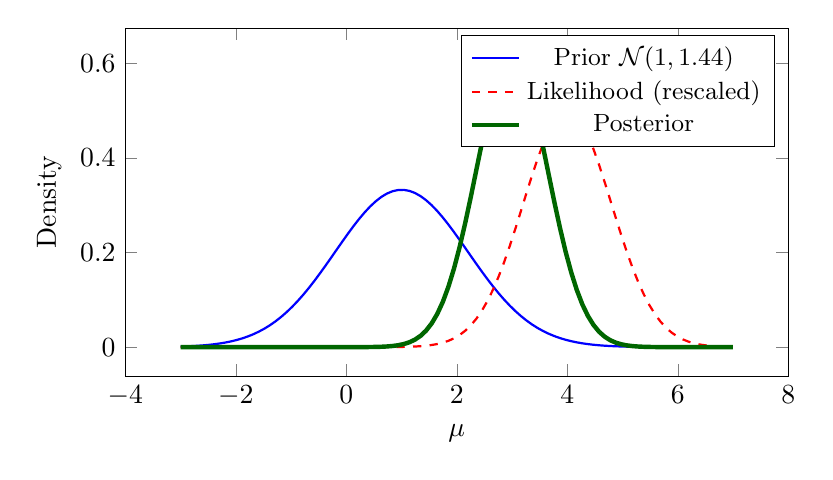
\begin{tikzpicture}[
    declare function={
      gauss(\x,\m,\s) = exp(-(\x-\m)^2/(2*\s*\s))/(sqrt(2*pi)*\s);
    }
  ]
  \begin{axis}[
    width=10cm, height=6cm,
    domain=-3:7, samples=100,
    xlabel=$\mu$, ylabel=Density,
    legend style={at={(0.98,0.98)}, anchor=north east, font=\small},
    no markers
  ]
    \addplot[blue, thick]{gauss(x,1,1.2)};
    \addlegendentry{Prior $\mathcal{N}(1, 1.44)$}
    \addplot[red, thick, dashed]{gauss(x,4,0.8)};
    \addlegendentry{Likelihood (rescaled)}
    \addplot[black!60!green, ultra thick]{gauss(x,3.0,0.65)};
    \addlegendentry{Posterior}
  \end{axis}
\end{tikzpicture}
\caption{Bayesian updating: the posterior (green) is a compromise between the prior (blue) and the likelihood (red, dashed). With more data, the posterior shifts towards the MLE.}
\label{fig:prior-posterior}
\end{figure}

%% ----------------------------------------------------------------
\section{Bayesian Linear Regression}

Consider the model $y = \bm{w}^\top\bm{x}+\epsilon$, $\epsilon\sim\mathcal{N}(0,\sigma^2)$, with prior $\bm{w}\sim\mathcal{N}(\bm{0},\tau^2\bm{I})$.

\begin{theorem}[Bayesian Linear Regression Posterior]
Given data $\bm{X}\in\R^{n\times p}$ and $\bm{y}\in\R^n$, the posterior of $\bm{w}$ is Gaussian:
\[
  p(\bm{w}\mid\bm{X},\bm{y}) = \mathcal{N}(\bm{w}\mid\bm{m}_n,\bm{S}_n),
\]
with
\begin{align}
  \bm{S}_n &= \bigl(\sigma^{-2}\bm{X}^\top\bm{X} + \tau^{-2}\bm{I}\bigr)^{-1}, \\
  \bm{m}_n &= \sigma^{-2}\bm{S}_n\bm{X}^\top\bm{y}.
\end{align}
\end{theorem}

\begin{proof}
The log-posterior is (up to a constant):
\begin{align}
  \ln p(\bm{w}\mid\bm{X},\bm{y})
  &= -\frac{1}{2\sigma^2}\norm{\bm{y}-\bm{X}\bm{w}}^2 - \frac{1}{2\tau^2}\norm{\bm{w}}^2 + \text{const} \\
  &= -\frac{1}{2}\bm{w}^\top\bigl(\sigma^{-2}\bm{X}^\top\bm{X}+\tau^{-2}\bm{I}\bigr)\bm{w}
     + \bm{w}^\top\sigma^{-2}\bm{X}^\top\bm{y} + \text{const}.
\end{align}
Completing the square in $\bm{w}$ gives the stated Gaussian form.
\end{proof}

\begin{definition}[Predictive Distribution]
For a new input $\bm{x}_*$, the predictive distribution is
\[
  p(y_*\mid\bm{x}_*,\mathcal{D})
  = \mathcal{N}\bigl(\bm{m}_n^\top\bm{x}_*,\;\sigma^2 + \bm{x}_*^\top\bm{S}_n\bm{x}_*\bigr).
\]
The predictive variance has two components: observation noise $\sigma^2$ and \emph{epistemic} uncertainty $\bm{x}_*^\top\bm{S}_n\bm{x}_*$ (which shrinks as data grows).
\end{definition}

%% ----------------------------------------------------------------
\section{Gaussian Processes}

\begin{definition}[Gaussian Process]
A \emph{Gaussian process} (GP) is a collection of random variables, any finite subset of which has a joint Gaussian distribution. A GP is fully specified by its mean function $m(\bm{x})$ and covariance (kernel) function $\kappa(\bm{x},\bm{x}')$:
\[
  f \sim \mathcal{GP}\bigl(m(\bm{x}),\,\kappa(\bm{x},\bm{x}')\bigr).
\]
\end{definition}

\subsection{Common Kernels}

\begin{keyformulas}[title=\textbf{GP Kernel Functions}]
\begin{itemize}
  \item \textbf{Squared Exponential (RBF)}:
    $\kappa(\bm{x},\bm{x}')=\sigma_f^2\exp\!\bigl(-\frac{\norm{\bm{x}-\bm{x}'}^2}{2\ell^2}\bigr)$
  \item \textbf{Mat\'ern $\nu=5/2$}:
    $\kappa(\bm{x},\bm{x}')=\sigma_f^2\bigl(1+\frac{\sqrt{5}\,r}{\ell}+\frac{5r^2}{3\ell^2}\bigr)\exp\!\bigl(-\frac{\sqrt{5}\,r}{\ell}\bigr)$,\; $r=\norm{\bm{x}-\bm{x}'}$
  \item \textbf{Rational Quadratic}:
    $\kappa(\bm{x},\bm{x}')=\sigma_f^2\bigl(1+\frac{\norm{\bm{x}-\bm{x}'}^2}{2\alpha\ell^2}\bigr)^{-\alpha}$
  \item \textbf{Periodic}:
    $\kappa(\bm{x},\bm{x}')=\sigma_f^2\exp\!\bigl(-\frac{2\sin^2(\pi\norm{\bm{x}-\bm{x}'}/T)}{\ell^2}\bigr)$
\end{itemize}
\end{keyformulas}

\subsection{GP Regression}

\begin{theorem}[GP Posterior]
Given training data $(\bm{X},\bm{y})$ with noise model $y=f(\bm{x})+\epsilon$, $\epsilon\sim\mathcal{N}(0,\sigma_n^2)$, the posterior over function values $\bm{f}_*$ at test inputs $\bm{X}_*$ is
\[
  \bm{f}_*\mid\bm{X}_*,\bm{X},\bm{y} \;\sim\; \mathcal{N}(\bar{\bm{f}}_*,\,\operatorname{cov}(\bm{f}_*)),
\]
where
\begin{align}
  \bar{\bm{f}}_* &= \bm{K}_{*}\bigl(\bm{K}+\sigma_n^2\bm{I}\bigr)^{-1}\bm{y}, \label{eq:gp-mean}\\
  \operatorname{cov}(\bm{f}_*) &= \bm{K}_{**} - \bm{K}_{*}\bigl(\bm{K}+\sigma_n^2\bm{I}\bigr)^{-1}\bm{K}_{*}^\top, \label{eq:gp-cov}
\end{align}
with $\bm{K}=\kappa(\bm{X},\bm{X})$, $\bm{K}_*=\kappa(\bm{X}_*,\bm{X})$, $\bm{K}_{**}=\kappa(\bm{X}_*,\bm{X}_*)$.
\end{theorem}

\begin{remark}
GP regression is equivalent to Bayesian linear regression in the (possibly infinite-dimensional) feature space induced by the kernel $\kappa$.
\end{remark}

\begin{figure}[ht]
\centering
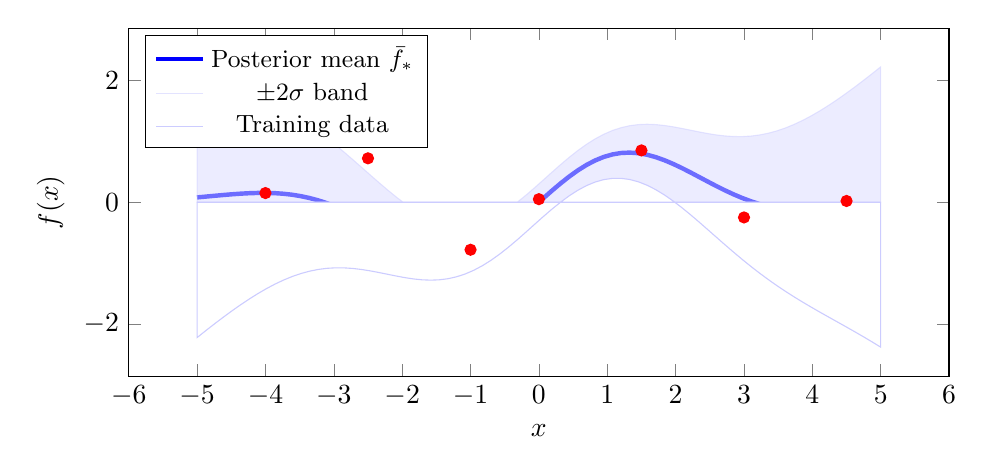
\begin{tikzpicture}
  \begin{axis}[
    width=12cm, height=6cm,
    xlabel=$x$, ylabel=$f(x)$,
    legend style={at={(0.02,0.98)}, anchor=north west, font=\small},
    no markers
  ]
    % Posterior mean
    \addplot[blue, ultra thick, domain=-5:5, samples=80]{sin(deg(x))*exp(-0.1*x*x)};
    \addlegendentry{Posterior mean $\bar{f}_*$}
    % Confidence band (approximate)
    \addplot[blue!20, fill=blue!15, opacity=0.5, domain=-5:5, samples=80]
      {sin(deg(x))*exp(-0.1*x*x)+0.3+0.08*x*x} \closedcycle;
    \addplot[blue!20, fill=white, domain=-5:5, samples=80]
      {sin(deg(x))*exp(-0.1*x*x)-0.3-0.08*x*x} \closedcycle;
    \addlegendentry{$\pm 2\sigma$ band}
    % Training points
    \addplot[only marks, mark=*, mark size=2pt, red]
      coordinates {(-4,0.15) (-2.5,0.72) (-1,-.78) (0,0.05) (1.5,.85) (3,-.25) (4.5,.02)};
    \addlegendentry{Training data}
  \end{axis}
\end{tikzpicture}
\caption{GP regression: the posterior mean interpolates the training points (red dots), and the uncertainty band widens away from observed data.}
\label{fig:gp-regression}
\end{figure}

%% ----------------------------------------------------------------
\section{Implementation in Python}

\begin{codeblock}[title=\textbf{Bayesian Linear Regression}]
\begin{minted}{python}
import numpy as np
import matplotlib.pyplot as plt

np.random.seed(42)

# Generate data
n, sigma = 30, 0.5
X = np.sort(np.random.uniform(-3, 3, n))
y = 1.5 * X - 0.8 + sigma * np.random.randn(n)

# Design matrix (with intercept)
Phi = np.column_stack([np.ones(n), X])
p = Phi.shape[1]

# Prior: w ~ N(0, tau^2 I)
tau = 2.0
S0_inv = np.eye(p) / tau**2

# Posterior
Sn_inv = S0_inv + Phi.T @ Phi / sigma**2
Sn = np.linalg.inv(Sn_inv)
mn = Sn @ (Phi.T @ y / sigma**2)

print(f"Posterior mean: w0 = {mn[0]:.3f}, w1 = {mn[1]:.3f}")
print(f"Posterior std:  w0 = {np.sqrt(Sn[0,0]):.3f}, "
      f"w1 = {np.sqrt(Sn[1,1]):.3f}")

# Predictive distribution
X_test = np.linspace(-4, 4, 200)
Phi_test = np.column_stack([np.ones_like(X_test), X_test])
y_pred = Phi_test @ mn
y_var = sigma**2 + np.sum(Phi_test @ Sn * Phi_test, axis=1)

plt.figure(figsize=(8, 5))
plt.scatter(X, y, c="red", s=20, label="Data")
plt.plot(X_test, y_pred, "b-", label="Posterior mean")
plt.fill_between(X_test, y_pred - 2*np.sqrt(y_var),
                 y_pred + 2*np.sqrt(y_var),
                 alpha=0.2, color="blue", label=r"$\pm 2\sigma$")
plt.legend(); plt.xlabel("x"); plt.ylabel("y")
plt.title("Bayesian Linear Regression")
plt.savefig("figures/ch10_bayesian_linreg.pdf")
\end{minted}
\end{codeblock}

\begin{codeblock}[title=\textbf{Gaussian Process Regression with scikit-learn}]
\begin{minted}{python}
from sklearn.gaussian_process import GaussianProcessRegressor
from sklearn.gaussian_process.kernels import RBF, WhiteKernel

# Kernel: RBF + noise
kernel = 1.0 * RBF(length_scale=1.0) + WhiteKernel(noise_level=0.25)

gp = GaussianProcessRegressor(kernel=kernel, n_restarts_optimizer=10,
                                random_state=42)
gp.fit(X.reshape(-1, 1), y)

X_star = np.linspace(-4, 4, 200).reshape(-1, 1)
y_mean, y_std = gp.predict(X_star, return_std=True)

print(f"Optimised kernel: {gp.kernel_}")
print(f"Log-marginal-likelihood: {gp.log_marginal_likelihood_value_:.2f}")

plt.figure(figsize=(8, 5))
plt.scatter(X, y, c="red", s=20, zorder=5, label="Data")
plt.plot(X_star, y_mean, "b-", label="GP mean")
plt.fill_between(X_star.ravel(),
                 y_mean - 2*y_std, y_mean + 2*y_std,
                 alpha=0.2, color="blue", label=r"$\pm 2\sigma$")
plt.legend(); plt.xlabel("x"); plt.ylabel("y")
plt.title("GP Regression")
plt.savefig("figures/ch10_gp_regression.pdf")
\end{minted}
\end{codeblock}

%% ----------------------------------------------------------------
\section{Exercises}

\begin{exercise}[Beta--Binomial Conjugacy]
You flip a coin $n=20$ times and observe $k=13$ heads. Using a $\text{Beta}(1,1)$ (uniform) prior on the bias $\theta$, compute the posterior distribution, the posterior mean, the MAP estimate, and a 95\% credible interval. Compare with the MLE.
\end{exercise}

\begin{exercise}[Bayesian Linear Regression Posterior]
Derive the posterior $p(\bm{w}\mid\bm{X},\bm{y})$ for Bayesian linear regression by completing the square in the log-posterior. Verify that the posterior mean $\bm{m}_n$ equals the ridge regression solution with $\lambda=\sigma^2/\tau^2$.
\end{exercise}

\begin{exercise}[GP Kernel Design]
Using \texttt{scikit-learn}, fit GP regression models to $f(x)=\sin(2\pi x)$ with $n=20$ noisy observations. Compare the following kernels: (a) RBF, (b) Mat\'ern $\nu=3/2$, (c) RBF + Periodic. Plot the posterior mean and 95\% bands for each. Which kernel best captures the periodicity?
\end{exercise}

\begin{exercise}[Effect of Prior Strength]
In Bayesian linear regression, fix $\sigma^2=1$ and vary $\tau^2\in\{0.01,0.1,1,10,100\}$. For each, plot the posterior mean function and the 95\% predictive band. Describe how the prior strength affects the fit and the uncertainty.
\end{exercise}

\begin{exercise}[GP Marginal Likelihood]
For GP regression, the log-marginal-likelihood is
\[
  \ln p(\bm{y}\mid\bm{X},\bm{\theta})
  = -\tfrac{1}{2}\bm{y}^\top(\bm{K}+\sigma_n^2\bm{I})^{-1}\bm{y}
  - \tfrac{1}{2}\ln|\bm{K}+\sigma_n^2\bm{I}| - \tfrac{n}{2}\ln 2\pi.
\]
Implement this from scratch. Optimise the length-scale $\ell$ and signal variance $\sigma_f^2$ by gradient ascent. Compare with scikit-learn's automatic optimisation.
\end{exercise}
